\chapter{半空间弹性波散射问题}\label{chap:Elastic}
为了研究半空间弹性波反散射问题, 我们得先来研究正文题。
\section{半空间弹性波 Green 函数}\label{Green Tensor}
\subsection{Neumann Green 函数}\label{Neumann Green Tensor}
设源点$y\in\R^2_+$, 引入半空间弹性波Neumann零边界格林函数$\N(x,y)$, 对任意向量$q\in\R^2$, 其满足如下方程:
\be
& & \Delta_e [\N(x;y)q] + \omega^2 [\N(x,y)q] = -\mathbf{\delta}_y(x) q \ \ \mbox{in }\R^2_+ , \label{eq_n1} \\
& & \sigma(\N(x,y)q)e_2 = 0 \ \ \mbox{on } \Gamma_0, \label{eq_n2}
\ee
其中(\ref{eq_n2})代表该green函数满足半空间自由边界条件,${\delta}_y(x)$代表位于点y的Dirac源。 由于半空间的特性,我们将利用对$x_1$变量作Fourier变换的方式来推导Green函数,令
\be\label{a1}
\hat \N(\xi,x_2;y_2)= \int_\R\N(x_1,x_2;y) e^{-\i (x_1-y_1)\xi} dx_1,\ \ \forall \xi\in\C,
\ee
记 $\G(x,y)$ \cite{ku63} 为弹性波方程的基本解, 且对其$x_1$变量做Fourier变换后有
$\hat{\G}(\xi,x_2;y_2)=\hat{\G}_s(\xi,x_2;y_2)+\hat{\G}_p(\xi,x_2;y_2)$及
\be
& &\hat{\G}_s(\xi,x_2;y_2)=\frac{\i}{2\omega^2}
\left( \begin{array}{cc}
	\mu_s & -\xi\frac{x_2-y_2}{|x_2-y_2|} \\
	-\xi\frac{x_2-y_2}{|x_2-y_2|} & \frac{\xi^2}{\mu_s}
\end{array} \right)e^{\i\mu_s|x_2-y_2|}, \label{G1}\\
& &\hat{\G}_p(\xi,x_2;y_2)=\frac{\i}{2\omega^2} 
\left( \begin{array}{cc}
	\frac{\xi^2}{\mu_p} & \xi\frac{x_2-y_2}{|x_2-y_2|} \\
	\xi\frac{x_2-y_2}{|x_2-y_2|} & \mu_p
\end{array} \right) e^{\i\mu_p|x_2-y_2|}.\label{G2}
\ee
这里$\mu_\alpha=(k_\alpha^2-\xi^2)^{1/2}$且有$\alpha=s,p$, $k_p=\omega/\sqrt{\lam+2\mu}, k_s=\omega/\sqrt{\mu}$为p波和s波的波数。
为了利用基本解$\G(x,y)$的特性,我们令:
\ben
\N_c(x,y)=\N(x,y)-(\G(x,y)-\G(x,y'))
\een
其中$y'=(y_1,-y_2)$ 为y关于$x_1$轴的镜像点。于是由式(\ref{eq_n1}-\ref{eq_n2}),得$\N_c(x,y)$满足如下方程:
\be
& & \Delta_e [\N_c(x;y)q] + \omega^2 [\N_c(x,y)q] = 0 \ \ \mbox{in }\R^2_+ , \label{eq_n3} \\
& & \sigma(\N_c(x,y)q)e_2 =-\sigma(\G(x,y)-\G(x,y')) \ \ \mbox{on } \Gamma_0, \label{eq_n4}
\ee
\begin{remark}
	在全篇论文中,我们假设对于任意的$z\in \mathbb{C}\backslash\{0\}$, $z^{1/2}$是多值函数$\sqrt{z}$ 的如下解析分支:$\Im(z^{1/2})\geq 0$,这对应于在复平面取右半实轴为割支线。则对于$z=z_1+\mathbf{i}z_2$, $z_1,z_2\in\R$,
	\be \label{convention_1}
	z^{1/2}={\rm sgn}(z_2)\sqrt{\frac{|z|+z_1}{2}}+\i\sqrt{\frac{|z|-z_1}{2}},\ \ \forall z\in\C\backslash\bar{\R}_+.
	\ee
	当$z$位于右半实轴的上沿或是下沿时,取$z^{1/2}$为$\ep\rightarrow0^+$ 时$(z+\i\ep)^{1/2}$ 或是 $(z-\i\ep)^{1/2}$的极限即可。
\end{remark}

通过对式(\ref{eq_n3}-\ref{eq_n4})两边作Fourier变换,我们得到关于变量$x_2$的常系数常微分方程组:
\be
 \mu \frac{d^2(e_1^T\hat \N_c q)}{dx_2^2}+\i(\lambda+\mu)\xi\frac{d(e_2^T\hat \N_c q)}{dx_2}+(\omega^2-(\lambda+2\mu)\xi^2)(e_1^T\hat \N_c q) = 0 \label{eq_n5}\\
 (\lambda+2 \mu)\frac{d^2(e_2^T\hat \N_c q)}{dx_2^2}+\i(\lambda+\mu)\xi\frac{d(e_1^T\hat \N_c q)}{dx_2}+(\omega^2-\mu \xi^2)(e_2^T\hat \N_c q) = 0 \label{eq_n6}
\ee
 由于我们需要$\N(x,y)$为外行波解,因此方程 (\ref{eq_n5})的解为如下两个向量:
\ben
 \left[ \begin{array}{cc} \i\mu_s \\ -\i\xi \end{array} \right]e^{\i\mu_s x_2} \ , \ \ \ \ \ \left[ \begin{array}{cc} \i\xi \\ \i\mu_p \end{array} \right]e^{\i\mu_p x_2}
\een
的线性组合。 利用边界条件(\ref{eq_n6})及待定系数法,我们得到:
\be\label{NGT}
\hspace{-2cm}\hat \N_c(\xi,x_2;y_2) =  \frac{\i}{\omega^2\delta(\xi)}\sum_{\alpha,\beta=p,s}\mathbb{A}_{\al\beta}(\xi)e^{\i(\mu_\al x_2+\mu_{\beta} y_2)}, 
\ee
其中 $\varphi(\xi)=k_s^2-2\xi^2$, $\delta(\xi)=\varphi(\xi)^2+4\xi^2\mu_s\mu_p $(Rayleigh方程\cite{achenbach1980}), 以及 

\ben
&&{\mathbb{A}_{ss}(\xi)} =
\left( \begin{array}{ll}
	\varphi^2\mu_s & -4\xi^3\mu_s\mu_p \\
	-\xi\varphi^2  & 4\xi^4\mu_p
\end{array} \right),\ \ 
{\mathbb{A}_{sp}(\xi)} =
\left( \begin{array}{ll}
	2\xi^2\varphi\mu_s & -2\xi\varphi\mu_s\mu_p \\
	-2\xi^3\varphi  & 2\xi^2\varphi\mu_p
\end{array} \right),\\ 
\\
\\
&&
{\mathbb{A}_{ps}(\xi)} =
\left( \begin{array}{ll}
	2\xi^2\varphi\mu_s & 2\xi^3\varphi \\
	2\xi\varphi\mu_s\mu_p  & 2\xi^2\varphi\mu_p
\end{array} \right),\ \ 
{\mathbb{A}_{pp}(\xi)} =
\left( \begin{array}{ll}
	4\xi^4\mu_s & \xi\varphi^2 \\
	4\xi^3\mu_s\mu_p  & \varphi^2\mu_p
\end{array} \right).
\een
按照惯例,原本我们只要对$\hat{\N}(\xi,x_2;y_2)$进行Fourier逆变换就可以得到所需要的Neumann Green函数. 然而,如下面的引理所述, 函数$\delta(\xi)$在实轴上存在零点\cite{achenbach1980, Harris2001Linear},此时我们并不可以对其直接进行Fourier逆变换.
\begin{lem} \label{rayleigh}
	 Rayleigh方程 $\delta(\xi) = 0$在复平面$\C$中有且仅有两个根且记为 $\pm k_R$, 其中$k_R$满足$k_R>k_s$。
\end{lem}

\debproof
 由前文注记中的(\ref{convention_1}), 易得 $\delta(\xi)$ 的割支线为 $C_l=\{\xi=\xi_1+\i\xi_2\in\C: \xi_1\in [-k_s,-k_p],\xi_2=0\}$ 和 
$C_r=\{\xi=\xi_1+\i\xi_2\in\C: \xi_1\in [k_p,k_s],\xi_2=0\}$. 于是$\delta(\xi)$在除 $C_l$ 和 $C_r$ 以外的区域解析。 而在割支线上,$\delta(\xi)$ 可表示成: 
\ben
\delta(\xi)=(k_s^2-2\xi^2)^2+\i\,[4\xi^2(k_s^2-\xi^2)^{1/2}(\xi^2-k_p^2)^{1/2}], \ \ \forall \xi\in C_l\cup C_r.
\een
显然, $\de(\xi)$ 在 $C_l\cup C_r$ 上没有零点。 又因为 $\de(\pm k_s)>0$ , $\de(\pm\infty)<0$ ,由函数的连续性得 $\de(\xi)$ 在区间 $(-\infty,-k_s)\cup(k_s,\infty)$ 上至少存在两个零点, 且由于其对称性,可以记为 $\pm k_R$。 下面, 我们将 $C_l, \ C_r$ 的上下沿分别记为 $C_l^\pm, \ C_r^\pm$。

接下去, 利用幅角原理\cite{Ahlfors1979Complex}可以说明 $\delta(\xi)$ 在整个复平面只存在两个零点。 令 $\Ga_R$ 为半径 $R$ 充分大的圆. 我们考虑 $\mathcal D$ 是被周线 $\Ga_R$, $\Ga_l$ 以及 $\Ga_r$ 包围的区域。 其中 $\Ga_l$ 代表沿着 $C_l^+$ 从 $-k_s$ 到 $-k_p$  及然后沿着 $C_l^-$ 从 $-k_p$ 到 $-k_s$ ; 相应地, $\Ga_r$ 代表 沿着 $C_r^+$ 从 $k_p$ 到 $k_s$ 及然后 沿着 $C_r^-$ 从 $k_s$ 到 $k_p$ 。 因为 $\delta(\xi)$ 在整个整个复平面上没有极点,  我们可以通过幅角原理来计算其在区域
 $\mathcal D$ 中的零点个数 $Z$ :
\be\label{zero}
Z=\frac{1}{2\pi\i}\int_C \frac{\delta'(\xi)}{\delta(\xi)}d\xi.
\ee
由式子(\ref{convention_1})中的定义,我们可以得出当$\xi\in C_r^\pm$时 $\de(\xi)=\de^\pm(\xi)$, 其中
\ben
\de^\pm(\xi)=(k_s^2-2\xi^2)^2\mp\i\,[4\xi^2(k_s^2-\xi^2)^{1/2}(\xi^2-k_p^2)^{1/2}\,]:=f_1(\xi)\mp\i f_2(\xi).
\een
于是可以有如下计算
\ben
\int_{\Ga_r} \frac{\delta'(\xi)}{\delta(\xi)}d\xi&=&\int_{k_p}^{k_s}\left(\frac{{\delta}_{+}' (\xi)}{\delta_{+}(\xi)}-\frac{{\delta}_{-}' (\xi)}{\delta_{-}(\xi)}\right) d\xi\\
&=&2\i\int_{k_p}^{k_s}\frac{f_1'(\xi) f_2(\xi)-f_1(\xi) f_2'(\xi)}{f_1^2(\xi)+ f_2^2(\xi)} d\xi\\
&=&-2\i\arctan \frac{f_2(\xi)}{f_1(\xi)}\Bigg|^{k_s}_{k_p}=0.
\een
相似地, 在 $\xi\in C_r^\pm$ 时也有 $\int_{\Ga_l}\frac{\delta'(\xi)}{\delta(\xi)}d\xi=0$ 。 此外, 当 $|\xi|$ 足够大, 容易得到 $\de(\xi)$ 的渐近形式 $\delta(\xi)=-2(k_s^2-k_p^2)\xi^2+O(1)$ 及  。 于是当 $R\gg 1$ ,可以计算得到
$\int_{\Ga_R} \frac{\delta'(\xi)}{\delta(\xi)}d\xi=4\pi\i$ 。
综上所述, 我们得出 $Z=2$ 。 于是该引理得到证明。
\finproof


为了克服上述问题,我们先假设半空间的介质是耗散的,然后研究其相应的Green函数,最后通过极限吸收原理得到$\N(x,y)$。
记 $\mathbb{N}_{\omega(1+\i\ep)}(x,y)$ 为满足将式子(\ref{eq_n1})中将实圆频率$\omega$ 替换为复圆频率$\om(1+\i\ep)$后相应方程的Green函数。 同样的, 对$\mathbb{N}_{\omega(1+\i\ep)}(x,y)$关于$x_2$变量的Fourier变换,得到$\hat\N_{\omega(1+\i\ep)}(\xi,x_2;y_2)$,且通过相同的推导,其表达式与将(\ref{NGT})中将$k_s, k_p$替换为
$k_s(1+\i\ep), k_p(1+\i\ep)$后相应的式子一致。 下面的两个引理告诉我们,$\hat\N_{\omega(1+\i\ep)}(\xi,x_2;y_2)$的零点所在何处。

\begin{remark}
	通篇全文中, 我们都假设耗散介质中所添加的 $\i\ep$ 是足够小的。
\end{remark}
对于 $\al=s,p$, 令$\mu_{\al,\ep}(\xi)=((k_\al(1+\i\ep))^2-\xi^2)^{1/2}$。于是, 根据规定 (\ref{convention_1}), 易得 $\mu_{\al,\ep}(\xi)$ 的割支线 $\mathcal{C_{\al,\ep}}$为
\ben
\mathcal{C_{\al,\ep}}&=&\{\xi=(\xi_1,\xi_2)\in\C \ | \ \Im \mu_{\al,\ep}(\xi)=0\} \\
&=&\{\xi=(\xi_1,\xi_2)\in\C \ | \   \xi_1\xi_2=k_\al^2\ep \ , \  \ \xi_2/\xi_1>\ep  \}
\een
如图 \ref{figure_cut} 所示。
\begin{figure}[htbp]
	\centering
	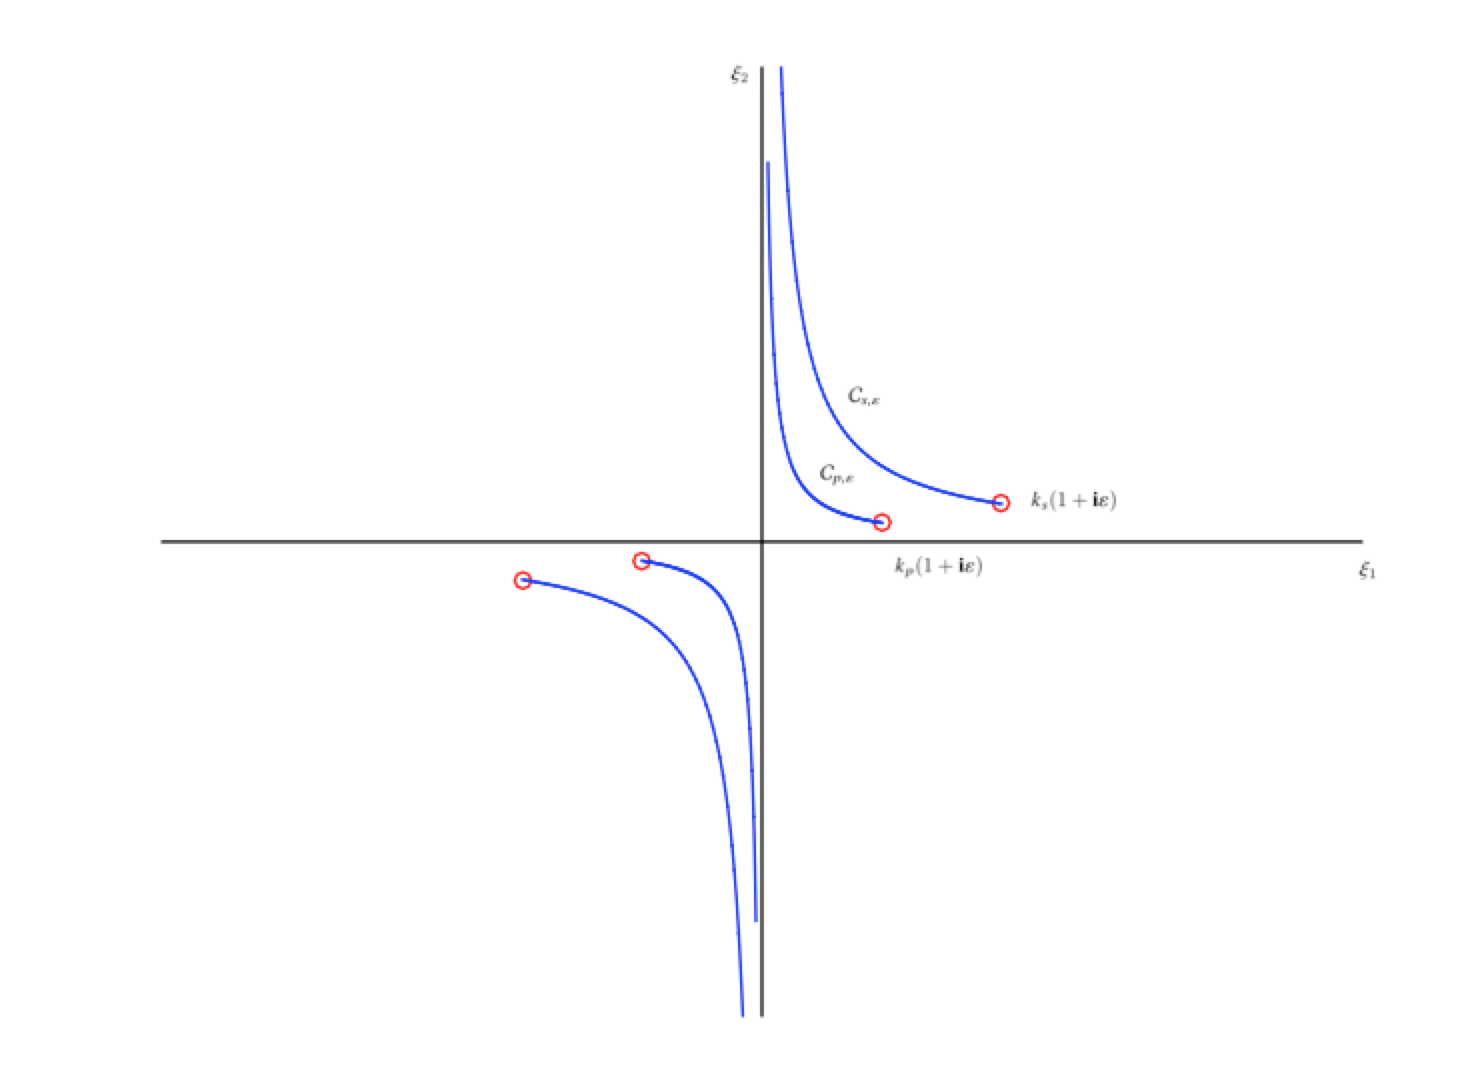
\includegraphics[width=\textwidth]{./Img/cut_plot}
	\caption{$\mu_{\al,\ep}(\xi)$, $\al=p,s$ 相应的割支线} \label{figure_cut}
\end{figure}

令$\delta_{\om(1+\i\ep)}(\xi)$为将$\delta(\xi)$中的$k_p,k_s$替换成$k_s(1+\i\ep),  k_p(1+\i\ep)$后相应的复Rayleigh方程。 为了展现 $\delta_{\om(1+\i\ep)}(\xi)$ 的零点 与 $\delta(\xi)$ 的零点的关系,我们先来刻画在何种情况下可以结合或是分离根式 $z^{1/2}$ 。
\begin{lem}\label{lem23}
	令 $0<\ep<1$ , 假设 $z=R e^{\i\phi}$, $(1+\i\varepsilon)=r e^{\i\psi}$ 其中有 $0\leq\phi<2\pi$, $0<\psi<\pi/2$ 和  $R,r>0$. 于是等式
	\be
	z^{1/2}=(1+\i\varepsilon)(\frac{z}{{1+\i\varepsilon}^2})^{1/2}
	\ee
	当且仅当  $2\psi\leq\phi<2\pi$
\end{lem}
\debproof
令 
\ben
z_\ep=z/(1+\i\ep)^2:=R_\ep e^{\i\phi_\ep},
\een
 其中 $0\leq\phi_\ep<2\pi$。于是,易得当 $2\psi\leq\phi<2\pi$ 时, 成立 
\ben
\phi_\ep=\phi-2\psi , \ R_\ep=R/r,
\een 
则有
\ben
z^{1/2}&=&\sqrt{R}e^{\i\phi/2}
=\sqrt{R/r}\sqrt{r}e^{\i(\phi/2-\psi)+\i\psi}\\
&=&\sqrt{R_\ep}\sqrt{r}e^{\i(\phi_\ep)+\i\psi}
=(1+\i\ep)z_\ep^{1/2}
\een
同样地, 当 $0\leq\phi<2\psi$ 时, 成立 
\ben
\phi_\ep=\phi-2\psi+2\pi
\een
 则有 
 \ben
 z^{1/2}=-(1+\i\ep)z_\ep^{1/2}.
 \een
  引理得证
\finproof

下面的引理告诉我们,$\hat\N_{\omega(1+\i\ep)}(\xi,x_2;y_2)$的零点所在何处。

\begin{lem}\label{complex_rayleigh}
	复Rayleigh方程 $\delta_{\om(1+\i\ep)}(\xi)$在$\C\bks{\Om}$中有且仅有两个根且为$\pm k_R(1+\i\ep)$。 其中集合$\Om$为
	\be\label{set:Om}
	\Omega := \{\xi_1+\i\xi_2 \in \mathbb{C} \ | \ k_p^2\ep<\xi_1\xi_2<k_s^2\ep \ , \  \ \xi_2/\xi_1>\ep\}
	\ee
\end{lem}
\debproof
 我们定义 
 \ben
 \mu_\ep=(k^2(1+\i\ep)^2-\xi^2)^{1/2},k\in\R^+,
 \een
  令 
  \ben
  \xi=\xi_1+\i\xi_2,\xi_1,\xi_2\in\R, \ \ \  (1+\i\varepsilon)=r e^{\i\psi}.
  \een
  通过简单的计算, 我们有
\be
\mu_\ep^2 &=& k^2(1-\ep^2)-\xi_1^2+\xi_2^2+\i(2k^2\ep-2\xi_1\xi_2)\\
&:=&Re^{\i\Theta} := a_1+\i a_2
\ee
定义 $\Delta:=\{ \xi | 2\psi\leq\Theta<2\pi \} $ , 于是由引理 \ref{lem23} , 当 $\xi \in\Delta$ 时,成立
\ben
\mu_\ep = (k^2-\xi_\ep^2)^{1/2} (1+\i\ep),
\een
另一方面当 $\xi \notin\Delta$ 时,成立 
\ben
 \mu_\ep = - (k^2-\xi_\ep^2)^{1/2} (1+\i\ep)
 \een
 其中 $\xi_\ep=\xi/(1+\i\ep)$。 由于 $\ep$ 足够小, 我们可以有如下关于集合 $\Delta$ 的等价形式:
\be\nn
\Delta &=& (\pi/2\geq\Theta<2\pi)\cup(2\psi<\Theta<\pi/2) \\ \label{setd}
&=& \{ \xi | a_1 \leq 0 \} \cup \{ \xi | a_2 \leq 0 \} \cup \{ \xi | a_1 >0,a_2 >0 \ ,\ \ \tan\Theta \geq \tan(2\psi) \} \\ \nn
&:=& \Delta_1 \cup \Delta_2 \cup \Delta_3
\ee
将 
\ben
& &a_1=k^2(1-\ep^2)-\xi_1^2+\xi_2^2 \\
& &a_2=(2k^2\ep-2\xi_1\xi_2)
 \een
  代入式子 (\ref{setd}) 中, 我们得到
\be
\Delta_1 &=& \{ \xi | \xi_1^2-\xi_2^2 \geq k^2(1-\ep^2) \}  \\
\Delta_2 &=& \{ \xi | \xi_1\xi_2 \geq k^2\ep \}
\ee
又由于 $\tan\Theta=a_1/a_2$, $\tan\psi=\ep$, 易得
\be
\Delta_3 = \{ \xi | \xi_1^2-\xi_2^2 \leq k^2(1-\ep^2), \xi_1\xi_2 \leq k^2\ep ,
\frac{k^2\ep-\xi_1\xi_2}{k^2(1-\ep^2)-(\xi_1^2-\xi_2^2)} \geq \frac{\ep}{1-\ep^2} \}
\ee
观察 $\Delta_3$ , 我们发现 $\Delta_3$ 表示成为 $\Delta_3=\Delta_{31}\cup\Delta_{32}\cup\Delta_{33}$ , 
其中
\ben
\Delta_{31} &=& \{ \xi | \xi_1\xi_2 \leq 0, 0\leq\xi_1^2-\xi_2^2 \leq k^2(1-\ep^2) \} \\
\Delta_{32} &=& \{ \xi |0 \leq \xi_1\xi_2 \leq k^2\ep, 0\leq\xi_1^2-\xi_2^2 \leq k^2(1-\ep^2), \frac{\xi_1\xi_2}{\xi_1^2-\xi_2^2} \leq \frac{\ep}{1-\ep^2} \} \\
&=& \{\xi | 0 \leq \xi_1\xi_2 \leq k^2\ep, 0\leq\xi_1^2-\xi_2^2 \leq k^2(1-\ep^2), \frac{\xi_2}{\xi_1} \leq \ep \} \\
\Delta_{33} &=& \{ \xi |\xi_1\xi_2 \leq 0, \xi_1^2-\xi_2^2 \leq 0 ,\frac{\xi_1\xi_2}{\xi_1^2-\xi_2^2} \geq \frac{\ep}{1-\ep^2} \} \\
&=& \{ \xi |\xi_1\xi_2 \leq 0, \xi_1^2-\xi_2^2 \leq 0 ,-\frac{\xi_1}{\xi_2} \geq \ep \}
\een
观察到 $\xi_1\xi_2 = k^2\ep$ , $\xi_1^2-\xi_2^2 = k^2(1-\ep^2)$ , $\xi_2=\xi_1\ep$ 三条曲线交于点 $\pm k(1+\i\ep)$, 于是区域 $\Delta$ 可以简化成:
\be
\Delta = \{\xi |-\frac{\xi_1}{\xi_2} \geq \ep, \ \frac{\xi_2}{\xi_1} \leq \ep\}\cup\{\xi | \xi_1\xi_2 \geq k^2\ep \}
\ee
定义 $\Delta_s,\Delta_p$ 为将 $\mu_\ep$ 中的 $k$ 替换为 $k_s,k_p$ 后相应的 $\Delta$ 区域。于是, 经过简单的整理, 我们可以得到:
\be
\C\bks\Omega = (\Delta_s \cap \Delta_p )\cup (\C\backslash(\Delta_s \cup \Delta_p))
\ee
因此,当 $\xi\in\C\bks\Omega$ , 成立
\ben
\delta_{\om(1+\i\ep)}=\delta(\xi_\ep)(1+\i\ep)^4 
\een
 通过引理 \ref{rayleigh} , 此引理得证。
\finproof

 由引理\ref{complex_rayleigh} 我们得知 $\hat\N_{\omega(1+\i\ep)}(\xi,x_2;y_2)$ 在实轴上没有极点, 可以对其直接进行逆Fourier变换。 于是,半空间弹性波 Neumann Green函数 $\mathbb{N}(x,y)$ 可以利用极限吸收原理得到,即为
\be\nn
\N(x,y)&=&\lim_{\ep\to 0^+} \N_{\om(1+\i\ep)}(x,y)\\ \label{NGT1}
&=&\lim_{\ep\to 0^+}\frac{1}{2\pi}\int_\R\hat \N_{\om(1+\i\ep)}(\xi,x_2;y_2) e^{\i(x_1-y_1)\xi} d\xi.
\ee

现在, 我们已经得到 Neumann Green 函数的具体表达形式了。 但是,式子(\ref{NGT1})中这种极限形式并不利于我们分析该函数的具体性质,特别是其无穷远处的衰减阶数。 为了便于得到更加易于分析的表达形式, 我们引入下面这个关于柯西主值(cf. e.g. \cite[Chapter 4, Theorem 5]{Kuroda})的引理
\begin{lem}\label{cauchy_pv}
	令 $a,b\in\R,\  a<b$, 且 $t_0\in (a,b)$. 如果 $\gamma$ 在$[a,b]$上 H\"older 连续, 即存在常数 $\alpha\in (0,1]$ 及 $C>0$ 对于任意 $s,t\in [a,b]$, $|\gamma(s)-\gamma(t)|\le C|s-t|^\alpha$, 于是有
	\ben
	\lim_{z\to t_0,\pm\Im z>0}\int^b_a\frac{\gamma(t)}{t-z}dt={\rm p.v.}\int^b_a\frac{\gamma(t)}{t-t_0}dt\pm\pi\i\ga(t_0),
	\een
	其中 ${\rm p.v.}\int^b_a$ 表示积分的Cauchy主值。
\end{lem}

通过引理 \ref{rayleigh}, 引理 \ref{complex_rayleigh} , 易知 $\hat\N_{\omega(1+\i\ep)}(\xi\mp k_R(1+\i\ep))$ 在点 $\pm k_R$ 的某个小领域内解析且
关于 $\ep$ 一致有界。 于是, 对于足够小的 $d>0$,  成立:
\be
& &\lim_{\ep\to 0^+}\int_{\pm k_R-d}^{\pm k_R+d}\hat \N_{\om(1+\i\ep)}(\xi,x_2;y_2) e^{\i(x_1-y_1)\xi} d\xi \\
&=& \lim_{\ep\to 0^+}\int_{\pm k_R-d}^{\pm k_R+d}\frac{\hat \N(\xi,x_2;y_2)(\xi-k_R)}{\xi\mp k_R(1+\i\ep)} e^{\i(x_1-y_1)\xi} d\xi
\ee

然后利用引理 \ref{cauchy_pv} , 表达式 (\ref{NGT1}) 及上面的等式, 可以得到如下 Neumann Green 函数的表达式:
\be\label{NGT2}
\N(x,y)&=&\frac{1}{2\pi}\,{\rm p.v.}\int_{\R}\hat \N(\xi,x_2;y_2) e^{\i(x_1-y_1)\xi} d\xi\\
& &-\frac{1}{2\omega^2}
\left[\sum_{\alpha,\beta=p,s}\frac{\mathbb{A}_{\al\beta}(\xi)}{\de'(\xi)}e^{\i(\mu_\al x_2+\mu_\beta y_2)+\i(x_1-y_1)\xi}\right]^{k_R}_{-k_R},\ \ \forall x,y\in\R^2_+,
\ee
这里 $[f(\xi)]^b_a:=f(b)-f(a)$ 。

\begin{remark}
	值得注意的是, 由于 $\hat\N(\xi,x_2;y_2)$ 在实轴上存在极点及研究目的的区别, 导致最终$\N(x,y)$可以存在多种等价的表达形式。 例如, 在文献 \cite{nedelec2011} 中 Duran 等人是利用 Cauchy 积分定理以及留数定理将积分路径从实轴变换到双曲线上, 从而避开被积函数的极点。 可以证明的是, 本文中推导出的 Green 函数与文献 \cite{nedelec2011} 中的是一致的。 
\end{remark}
\begin{remark}
从 Neumann Green 函数的表达式 (\ref{NGT2})中, 我们发现在第二项中, $\mu_{\al}(\pm k_R)=\i\sqrt{k_R^2-k_\al^2}$, 易知当 $x_2$ 增大时, 第二项的值是指数衰减的。所以,式 (\ref{NGT2}) 中第二项对应的波只在 $\Ga_0$ 附近以波数 $k_R$ 传播,当远离 $\Ga_0$时非常微弱, 且称为表面波 (Rayleigh 波) \cite{aki2002quantitative}。
\end{remark}

为了后文分析的便利, 我们给出以下引理, 叙述若干关于 Rayleigh 函数 $\delta(\xi)$ 的性质。

\begin{lem}\label{delta}
	令 $d_R=(k_R-k_s)/2$,其中 $k_R$ 为Rayleigh 表面波的波数。我们与如下结论: \\
	\rm{1}.对于任意 $|\xi|\le k_s+ d_R$, 存在只与 $\kappa$ 有关的常数 $C_1,C_2,C_3$,我们有
	 \ben
	 & & C_1k_s^4\le |\delta(\xi)|\le C_2k_s^4 \\
	 & &|\delta^{(k)}(\xi)|\le C_3(|k_s^2-\xi^2|^{-k+1/2}+|k_p^2-\xi^2|^{-k+1/2}),  \ \ \ \ k=1,2  
	 \een
	  \rm{2} 对于任意 $|\xi|\geq k_R$, 存在只与 $\kappa$ 有关的常数 $C$,我们有
	  \ben
	  |\de(\xi)|\ge Ck_s^2(|\xi|^2-k_R^2)
	  \een
	  \rm{3} 
	  令$\de(\xi)=\de_1(\xi)(\xi^2-k_R^2)$, 对于任意 $k_R-d_R\le |\xi|\le k_R+d_R$, 存在只与 $\kappa$ 有关的常数 $C$,我们有
	  \ben
	  |\de_1(\xi)|\ge Ck_s^2
	  \een
\end{lem}

\debproof
利用简单的求导计算,我们易得结论1。 
通过 Rayleigh 函数的定义, 有 $|\xi|\ge k_s$, $\de(\xi)=k_s^4f({\xi^2}/{k_s^2})$, 其中
\ben
f(t)=(2t-1)^2-4t\sqrt{t-1}\sqrt{t-\kappa^2},\ \ \forall t\ge 1.
\een
对于任意 $t\geq 1$, 易得:
\be\nn
f'(t)&=&8t-4-4\sqrt{t-1}\sqrt{t-\kappa^2}-2t\sqrt{t-1}/\sqrt{t-\kappa^2}-2t\sqrt{t-\kappa^2}/\sqrt{t-1}\\ \label{df}
&\leq& 8t -4 -4\sqrt{t-1}\sqrt{t-k_R^2}-4t 
\ee
显然,当 $t\to1, \ t>1$ 时,$f'(t)\to-\infty$, 于是存在$\delta>0$ 即 $A_1>0$, 当 $1<t<1+\delta$ 时, $f'(t)<-A_1$。 而当 $t\geq 1+\delta$ 时, 由式子 (\ref{df})得,存在 $A_2>0$ , 有$f'(t)\leq -A_2$
又因为 $f(1)=1$ 以及 $f((2-\kappa^2)/(1-\kappa^2))<0$ 。 于是立得 $k_R^2\le\frac{2-\kappa^2}{1-\kappa^2}k_s^2$ 。 然后由中值定理及 $f'(t)\leq -\max(A_1,A_2)$ 得
\ben 
\min_{|\xi|\ge k_s}|\frac{\de(\xi)}{\xi^2-k_R^2}|\ge\min_{t\geq1}|f'(t)|k_s^2\ge \max(A_1,A_2)k_s^2,
\een
结论2, 3得证。
\finproof

观察式子 (\ref{G1}) , (\ref{G2}) , 及 (\ref{NGT}), 通过简单的变量替换, 我们易得 Neumann Green 函数满足如下对称性或是空间互易性,即
\be\label{symm}
\N(x,y)=\N(y,x)^T \ \ \ \ \ \ \ \forall x,y\in\R^2_+
\ee
对于 $x_s\in\Ga_0$ 的情况, 我们定义这种 Green 函数 $\N(x,x_s),x\in\R^2_+$ 为 $\N(x,y)$ 在 $y\in\R^2_+,  \  y\to x_s$ 时的极限。
由于半空间反散射问题中的点源一般都位于界面上, 所以接下去我们重点研究 $x\in\Ga_0 ,  \ y\in\R^2_+$ 时的 Neumann Green 函数 $\N(x,y)$ 。
通过 (\ref{G1}) , (\ref{G2}) , (\ref{NGT}), 简单的计算可以简化 $\N(x,y)$ :
\be
\hat
\N(\xi,0;y_2)&=&\frac{\i}{\mu\delta(\xi)} \Bigg[ \Bigg(
\begin{array}{cc}
	2\xi^2\mu_s & -2\xi\mu_s\mu_p\\
	-\xi\varphi & \mu_p\varphi
\end{array} \Bigg)e^{\i\mu_p y_2} \\ \nn
& &
+ \Bigg(
\begin{array}{cc}
	\mu_s\varphi & \xi\varphi \\
	2\xi\mu_s\mu_p & 2\xi^2\mu_p
\end{array} \Bigg)e^{\i\mu_s y_2} \Bigg] \nonumber\\
&:=&\frac{1}{\delta(\xi)}(\Np(\xi)e^{\i\mu_p y_2}+\Ns(\xi)e^{\i\mu_s y_2}), \label{d2}
\ee
且, 当 $x\in\Ga_0, y\in\R^2_+$,
\be\label{c8}
\N(x,y)&=&\frac{1}{2\pi}\,{\rm p.v.}\int_{\R}\hat \N(\xi,0;y_2) e^{\i(x_1-y_1)\xi} d\xi \\ \nn
& &+\frac\i 2
\left[\sum_{\al=p,s}\frac{\Na(\xi)}{\de'(\xi)}e^{\i\mu_\al y_2+\i(x_1-y_1)\xi)}\right]^{k_R}_{-k_R}.
\ee

为了便于研究 Neumann Green 函数在边界 $\Ga_0$上水平方向的渐近行为, 我们下面引理中更为有用的表达形式。


\begin{lem}\label{lem:2.3} 令 $x\in\Ga_0 \ , y\in \R^2_+$ 以及 $\phi\in (-\pi/2,\pi/2)$ 且存在如下表达 $y_2=|x-y|\cos\phi \ ,
	x_1-y_1=|x-y|\sin\phi$ 。 假设 $x_1\not= y_1$, 于是可以得到
	\be
	\N(x,y)&=&\frac{1}{2\pi}\int_L\mathbb{N}_0(t)\cos(t+\phi)e^{\i\lam\cos t}dt \\
	\nn
	& & \pm\i
	\left[\sum_{\al=p,s}\frac{\Na(\xi)}{\de'(\xi)}e^{\i\mu_\al y_2+\i(x_1-y_1)\xi}\right]_{\xi=\pm k_R},\label{h3}
	\ee
	其中 $\lam=k_s|x-y|$, $L$ 为复平面中的积分路径即 从 $-\pi/2+\i\infty$ to $-\pi/2$, $-\pi/2$ 到 $\pi/2$, 接着从 $\pi/2$ 到 $\pi/2-\i\infty$  ( 见图例 \ref{figure_trans}), 这里符号 $\pm$ 取决于 ${\rm sgn}(x_1-y_1)=\pm 1$, 且定义表达式:
	\be\label{h2}
	\mathbb{N}_{0}(t)=\sum_{\al=p,s}k_s\,\frac{\Na(k_s\sin(t+\phi))}{\de(k_s(\sin(t+\phi))}.
	\ee
\end{lem}

\debproof
不失一般性, 我们可以假设 $x_1>y_1$, 因此有 ${\rm sgn}(x_1-y_1)=1$。 注意到 $\hat{\N}(\xi,0;y_2)=\sum_{\al=p,s}\frac{\Na(\xi)}{\de(\xi)}e^{\i (y_2\mu_\al+(x_1-y_1)\xi)}$,所以对于 $\al=p,s$, 我们可以做经典的三角变量替换, 即为 $\xi=k_\al\sin t$ 。 由于三角函数的周期性, 这里我们规定 $-\pi<\Re t \leq\pi$ 以保证变换的一一对应。 相应地, $\xi$ 在复平面中的积分路径 $\R$ 对应于 $t$ 所在复平面中的积分路径 $L$ 。 于是得到如下等式:
\ben
& &\frac{1}{2\pi}\,{\rm p.v.}\int_{\R}\hat \N(\xi,0;y_2) e^{\i(x_1-y_1)\xi} d\xi \\
&=&\frac 1{2\pi}\,{\rm p.v.}\int_L\sum_{\al=p,s}k_s\,\frac{\Na(k_s\sin t)}{\de(k_s\sin t)}\cos t\, e^{\i \lam\cos (t-\phi)}dt.
\een
令 $L_{-\phi}$ 为 $L$ 平移 $-\phi$ 后的积分路径, 立即得到
\be\label{h1}
& &\frac{1}{2\pi}\,{\rm p.v.}\int_{\R}\hat \N(\xi,0;y_2) e^{\i(x_1-y_1)\xi} d\xi \\
&=&\frac 1{2\pi}\,{\rm p.v.}\int_{L_{-\phi}}\mathbb{N}_0(t)\cos (t+\phi)\,e^{\i\lam\cos t}dt,
\ee
这里 $\mathbb{N}_0(t)$ 如 (\ref{h1}) 所定义。

设 $t_R\in L$ 满足等式 $k_R=k_s\sin t_R$, 于是 $k_R$ 即为 $t_R$ 在积分变换 $\xi=k_s\sin t$ 下的像点。 特别地, 由于 $k_R>k_s$, 则存在  $s_R>0$ 使得  $t_R=\pi/2-\i s_R\in L$ 。 对于任意$\ep>0$,令 $ L^\ep$ 表示如下积分路径: \ben
& &-\pi/2+\i\infty\to -\pi/2+\i (s_R+\ep)\cup\pa B^+_\ep(-t_R)\\
&\to& -\pi/2+\i(s_R-\ep)
\to -\pi/2
\to\pi/2\to\pi/2-\i(s_R-\ep)\\
&\to&\pa B^+_\ep(t_R)\to\pi/2-\i(s_R+\ep)\to\pi/2-\i\infty,
\een
 其中 $\pa B^+_\ep(\pm t_R)$ 表示圆心在 $\pm t_R$ 半径为 $\ep$ 的右半圆  (如图 \ref{figure_trans} 所示)。 然后, 令 $L^\ep_{-\phi}$ 为 $L^\ep$ 平移 $-\phi$ 后的积分路径。 于是, 利用 Cauchy 主值的定义及留数定理, 我们可以得知
\ben
& &\frac 1{2\pi}\,{\rm p.v.}\int_{L_{-\phi}}\mathbb{N}_0(t)\cos(t+\phi)\,e^{\i \lam\cos t}dt \\
&=&\lim_{\ep\to 0^+}\frac 1{2\pi}\int_{L^\ep_{-\phi}}\mathbb{N}_0(t)\cos (t+\phi)\,e^{\i \lam\cos t}dt\\
& &+\frac\i 2\sum_{t'=\pm t_R}{\rm Res}(\mathbb{N}_0(t)\cos (t+\phi)e^{\i \lam\cos t},t').
\een
\begin{figure}[htbp]
	\centering
	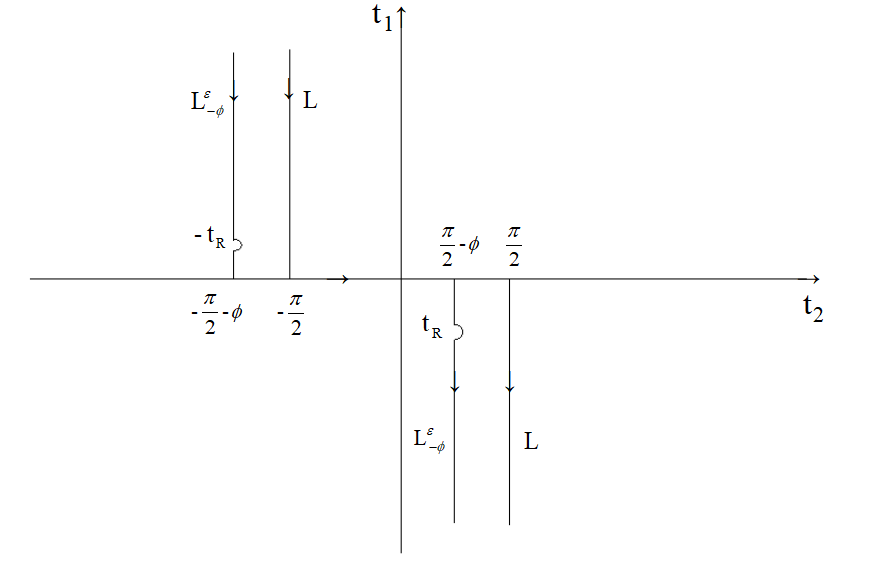
\includegraphics[width=\textwidth]{./Img/graphic/transformation4.png}
	\caption{ 积分路径 $L$ 和 $L^\ep_{-\phi}$}\label{figure_trans}
\end{figure}
通过简单的计算, 易得相应留数为:
\ben
& &\frac\i 2\sum_{t'=\pm t_R}{\rm Res}(\mathbb{N}_0(t)\cos (t+\phi)e^{\i \lam\cos t},t')\\
&=&\frac \i 2\sum_{\xi=\pm k_R}\sum_{\al=p,s}\frac{\Na(\xi)}{\de'(\xi)}e^{\i (y_2\mu_\al+(x_1-y_1)\xi)}.
\een
另一方面,通过 Cauchy 积分定理, 我们得到 
\ben
& &\frac 1{2\pi}\int_{L^\ep_{-\phi}}\mathbb{N}_0(t)\cos (t+\phi)\,e^{\i \lam\cos t}dt \\
&=&\frac 1{2\pi}\int_{L}\mathbb{N}_0(t)\cos (t+\phi)\,e^{\i \lam\cos t}dt.
\een
最后利用 (\ref{c8}) 和 (\ref{h1}) 引理得证。
\finproof
 
 上述引理是我们研究 Neumann Green 函数 $\N(x,y)$ 在界面 $\Ga_0$ 上当 $x\to\infty$ 时衰减行为估计的一个出发点。 下面, 我们先回顾下关于振荡积分衰减阶数估计的 Van der Corput 引理 \cite[P.152]{grafakos} 。
 
 \begin{lem}\label{van}
 	令 $\lam\ge 1$, $f\in C[a,b]$且其导函数绝对可积, 如果 $u\in C^k[a,b]$, 其中 $k\ge 1$ 及 $a<b$, 我们就有如下结论 \\
 	{\rm 1}. 如果 $|u'(t)|\ge 1$ 对于任意 $t\in (a,b)$ 成立,且 $u'$ 在 $(a,b)$ 上单调, 就断言
 	\ben
 	\left|\int^b_a f(t)e^{\i\lambda u(t)}dt\right|\le
 	3\lambda^{-1}\left(|f(b)|+\int^b_a |f'(t)|dt\right).
 	\een
 	{\rm 2}. 对于 $k\geq2$ 时, 如果 $|u^{(k)}(t)|\ge 1$ 对于任意 $t\in (a,b)$ 成立, 就断言 
 	\ben
 	\left|\int^b_a f(t)e^{\i\lambda u(t)}dt\right|\le
 	12k\lambda^{-1/k}\left(|f(b)|+\int^b_a|f'(t)|dt\right).
 	\een
 \end{lem}

在文献\cite{RTMhalf_aco}中,Chen 等对半空间逆时偏移算法的研究时,引理 \ref{van} 起到了关键的作用。该引理相对于驻相定理的优势在于,对于振幅函数 $f(t)$ 的光滑性要求更低,且对于 $\lambda$ 阶数的刻画具有一致性。然而, 当振幅函数具有弱奇异点时,直接使用引理 \ref{van} 就行不通了。 幸运的是,经过研究我们发现 当振幅函数存在弱奇异点, 且其与相位函数 $\phi(t)$ 的驻相点的距离存在正下界时, Van der corput 引理仍然成立,如下述引理刻画。


\begin{lem}\label{lem:2.5}
	令 $\lam\ge 1$, 假设$f\in C[-\pi/2,\pi/2]$ 且其导函数绝对可积。 于是对任意区间 $(a,b)\subset (-\pi/2,\pi/2)$, 可以得到
	\be\label{c1}
	\left|\int_a^bf(t)e^{\i\lam\cos t}dt\right| 
	\leq C\lam^{-1/2}\left(|f(0)|+\int_a^b|f'(t)|dt\right),
	\ee
	这里常数 $C$ 与 $a,b,\lam$ 及被积函数 $f$ 无关。 
	此外, 令 $\kappa\in (0,1)$ 以及 $\phi\in (-\pi/2,\pi/2)$ 满足条件 $|\phi|\geq\phi^*>\arcsin \kappa:=\phi_\kappa$ , 可以得到
	\be\label{c3}
	 & &\left|\int_{-\frac\pi 2}^{\frac\pi 2}f(t)(\kappa^2-\sin^2(t+\phi))^{-1/2}e^{\i\lam\cos t}dt\right|  \\ \nn
	&\leq& C\lam^{-1/2}\left(|f(0)|+\int_{-\frac\pi 2}^{\frac \pi2}|f'(t)|dt\right),
	\ee
	这里常数 $C$ 只与 $\phi^*$ 和 $\kappa$ 有关。
\end{lem}
\debproof
我们不妨假定 $\phi>0$ 。
其中估计 (\ref{c1}) 可以 \ref{van} 直接得到。 这是因为区间 $(a,b)$ 可以被切割成若干个互不相交的子区间, 并且在任意一个子区间上面 $\sin t$ 单调且 $|\sin t|$ 存在下界 $1/\sqrt 2$ 或是 $|\cos t|$ 存在下界 $1/\sqrt 2$ 。

令 $g(t)=\kappa^2-\sin^2(t+\phi)$ 。 由于 $0<\kappa<1$ $g(t)$, 易知 $g(t)$ 在区间 $(-\pi/2,\pi/2]$ 上有且仅有两个零点 $t_1, t_2$ , 而且可以求出
$t_1=\phi_\kappa-\phi$ 及 $t_2=-\phi_\kappa-\phi$ 或是 $t_2=\pi-\phi_\kappa-\phi$ , 这里 $t_2$ 取决于 $\phi+\phi_\kappa<\pi/2$ 或是 $\phi+\phi_\kappa\ge \pi/2$ 。 不失一般性, 我在后面的证明中都假设 $t_2=\pi-\phi_\kappa-\phi$ 。

令 $0<\ep_0 <\min(\frac{\phi^*-\phi_\kappa}{2},\frac{\phi_\kappa}{2})$ 。 显然成立 $t_1-\ep_0\geq -\pi/2, \ t_1+\ep_0\le -(\phi^*-\phi_\kappa)/2$ 以及 $t_2-\ep_0\ge(\phi^*-\phi_\kappa)/2$ 。于是, 我们可以把区间 $(-\pi/2,\pi/2)$ 切分成5个互补相交的子区间
\ben
& &I_1=(-\pi/2,t_1-\ep_0), \ I_2=(t_1-\ep_0,t_1+\ep_0), \\  
& &I_3=(t_1+\ep_0,t_2-\ep_0),  I_4=(t_2-\ep_0,t_2+\min(t_2+\ep_0,\pi/2)),\\ & &I_5=(\min(t_2+\ep_0,\pi/2),\pi/2)
\een
于是利用 (\ref{c1}) 可以得到
\be\label{c4}
& &  \left|\int_{I_1\cup I_3\cup I_5}f(t)(\kappa^2-\sin^2(t+\phi))^{-1/2}e^{\i\lam\cos t}dt\right| \\ \nn
&\leq& C\lam^{-1/2}\left(|f(0)|+\int_{-\frac\pi 2}^{\frac\pi 2}|f'(t)|dt\right),
\ee
其中常数 $C$ 只和 $\phi^*$ 及 $\kappa$ 有关。 

现在我们来估计在区间 $I_2, \ I_4$ 上的积分。 首先, 我们观察到, 在区间 $I_2\cup I_4$ 上成立不等式
 $|\sin t|\ge \sin((\phi^*-\phi_\kappa)/2)$ 。 此外在该区间上还成立,
 \ben
 |g'(t)|=|\sin(2(t+\phi))|\ge \min(\sin\phi_\kappa,\sin(\phi^*+\phi_\kappa))
 \een 
  令 $\de\in (0,\ep_0)$ 充分小,因为 $g(t_j)=0, j=1,2$, 于是利用中值定理, 对于任意 $t$ 满足 $ \de\le |t-t_j|\le \ep_0,j=1,2$ 我们有
\ben
\hspace{-1cm}|g(t)|\ge \min(\sin\phi_\kappa,\sin(\phi^*+\phi_\kappa))\de,\ \ 
\een
通过分部积分后,得到
\ben
& &\left|\int_{t_1-\ep_0}^{t_1-\de}f(t)g(t)^{-1/2}e^{\i\lam\cos t}dt\right| \\
&\le& C\delta^{-1/2}\lam^{-1}\left(|f(0)|+\int_{-\frac\pi 2}^{\frac \pi 2}|f'(t)|dt\right).
\een
类似地,
\ben
& &\left|\int_{t_1+\de}^{t_1+\ep_0}f(t)g(t)^{-1/2}e^{\i\lam\cos t}dt\right| \\
&\le& C\delta^{-1/2}\lam^{-1}\left(|f(0)|+\int_{-\frac\pi 2}^{\frac \pi 2}|f'(t)|dt\right).
\een
最后,我们可以得到 
\ben
& &\left|\int_{t_1-\delta}^{t_1+\de}f(t)g(t)^{-1/2}e^{\i\lam\cos t}dt\right| \\
&\leq&C\max_{t\in(-\pi/2,\pi/2)}|f(t)|\int_{-\delta}^{\de}|\kappa -\sin(\phi_\kappa+t)|^{-1/2}dt\\
&\leq&C\de^{1/2}\max_{t\in(-\pi/2,\pi/2)}|f(t)|.
\een
如此, 我们只要取 $\delta=\lam^{-1}$ 就可以得到
\ben
& &\left|\int_{I_2}f(t)(\kappa^2-\sin^2(t+\phi))^{-1/2}e^{\i\lam\cos t}dt\right| \\
&\leq& C\lam^{-1/2}\left(|f(0)|+\int_{-\frac\pi 2}^{\frac \pi 2}|f'(t)|dt\right).
\een
同理,在区间 $I_4$ 上的积分也可以被估计。 结合式子 (\ref{c4}) 中的估计, 引理得证。

\finproof

\begin{lem}\label{lem:2.7}
	令 $\phi\in (0,\pi/2)$ 以及 $H$ 表示双曲线 
	\ben
	\{\xi=\xi_1+\i\xi_2\in\C:(\xi_1/(k_s\cos\phi))^2-(\xi_2/(k_s\sin\phi))^2=1\}
	\een 
	定义 $f(\xi)$ 为 $H$ 领域上的解析函数。 于是, 存在只与 $\kappa$ 有关的常数 $C$, 成立
	\ben
	& &\left|\int_{L\bks [-\pi/2,\pi/2]}f(k_s\sin(t+\phi))e^{\i\lam\cos t}dt\right|\\
	& &+\left|\int_{L\bks [-\pi/2,\pi/2]}f(k_s\sin(t+\phi))\cos te^{\i\lam\cos t}dt\right|\\
	\hskip-2cm&\le&C\lam^{-1}(|f(0)|+\max_{\xi\in H}(k_s|f'(\xi)|)).
	\een 
\end{lem}

\debproof
注意到, 对于 $t=-\pi/2+\i s$, $s>0$ 有 $k_s\sin(t+\phi)=-\cosh(s)\cos\phi+\i\sinh(s)\sin\phi\in H$ 。 于是
\ben
I&= &\int_{-\pi/2}^{-\pi/2+\i\infty}f(k_s\sin(t+\phi))e^{\i\lam\cos t}dt\\
&=&\i\int^\infty_0f(-\cosh(s)\cos\phi+\i\sinh(s)\sin\phi)e^{-\lam\sinh(s)}ds
\een
于是, 利用分部积分就可以得到
\ben
|I|&=&|\int^\infty_0f(-\cosh(s)\cos\phi+\i\sinh(s)\sin\phi) /(-\lam\cosh(s)) \ de^{-\lam\sinh(s)}| \\
&\leq&\lam^{-1}(|f(0)|+\int^\infty_0|\frac{df(-\cosh(s)\cos\phi+\i\sinh(s)\sin\phi)/\cosh(s))} {ds}|e^{-\lam\sinh(s)}ds)
\een
 得到 $\pi/2\to\pi/2-\i\infty$ 上的积分值的估计。 于是, 不等式中的第一项估计得证。 类似地, 可以证明不等式中的第二项的估计。 引理得证。
\finproof

经过前述若干引理的铺垫, 我们下面给出当 $x\in\Gamma_0$, $y\in\R_+^2$ 时, Neumann Green 函数相对于变量 $x_1$ 的阶数估计。 

\begin{thm}\label{es_NGT}
	假定 $x\in\Gamma_0$, $y\in\R_+^2$ 且满足 $|x_1-y_1|/|x-y|\ge(1+\kappa)/2$ 及 $k_sy_2\ge 1$ 。存在只与 $\kappa$ 有关的常数 $C$ , 有如下估计
	\ben
	|\N(x,y)|+k_s^{-1}|\na_y\N(x,y)|\leq \frac{C}{\mu}\left(\frac{k_sy_2}{(k_s|x-y|)^{3/2}}+e^{-\sqrt{k_R^2-k_s^2}y_2}\right).
	\een
\end{thm}

\debproof 这里我们只证明关于 $\N(x,y)$ 的估计。 由于 $\na_y\N(x,y)$ 的函数特性和  $\N(x,y)$ 一直, 同理可证。   由引理 \ref{lem:2.3} 中的式子 (\ref{h3}) 启发, 不失一般性, 我们假定 $x_1>y_1$ , 即有 $\phi\in (0,\pi/2)$ 且满足 
\ben
\phi\ge\phi^*=\arcsin (1+\kappa)/2>\phi_\kappa
\een

 通过引理 \ref{delta} 中的结论 3 ,我们易得式子 (\ref{h3}) 中的第二项存在上界 $C\mu^{-1}e^{-\sqrt{k_R^2-k_s^2}y_2}$ , 即该项随着 $y_2$ 增大指数衰减。

针对式子 (\ref{h3}) 中的第一项,我们将其分成 p 波和 s 波两项:
\ben
& &\frac 1{2\pi}\int_L\mathbb{N}_0(t)\cos(t+\phi)e^{\i\lam\cos t}dt\\
&=&
\frac 1{2\pi}\int_L\sum_{\al=p,s} k_s\frac{\Na(k_s\sin(t+\phi))}{\de(k_s\sin(t+\phi))}\cos(t+\phi)e^{\i\lam\cos t}dt.
\een
由于, p 波和 s 波在表达形式上是相似的, 这里我们只分析含有 $[\Np(k_s\sin(t+\phi))]_{22}=\mu^{-1}(\varphi\mu_p)(k_s\sin(t+\phi))$ 这项, 然后另一项的分析就同理可得。 为了表达简便, 我规定如下表示
\ben
g(t)&=&k_s\frac{[\Np(k_s\sin(t+\phi))]_{22}}{\delta(k_s\sin(t+\phi))}\\
&:=&f(t)(\kappa^2-\sin^2(t+\phi))^{1/2}, \\ f(t)&=&\frac{k_s^2}{\mu}\frac{\varphi(k_s\sin(t+\phi))}{\de(k_s\sin(t+\phi))}.
\een
于是, 利用分部积分, 可以得到
\ben
& &\int_{L}g(t)\cos(t+\phi)e^{\i\lam\cos t}dt\\
&=&\cos\phi\int_Lg(t)\cos te^{\i\lam\cos t}dt-\sin\phi\int_{L}g(t)\sin te^{\i\lam\cos t}dt\\
&=&\cos\phi\int_Lg(t)\cos te^{\i\lam\cos t}dt-\frac{\sin\phi}{\i\lam}\int_{L}g'(t)e^{\i\lam\cos t}dt\\
&=&{\rm I}_1+{\rm I}_2.
\een
通过引理 \ref{delta} 中的结论 1 及引理 \ref{lem:2.5} 中的式 (\ref{c1}), 我们得到
\ben
& &\left|\int_{-\frac\pi 2}^{\frac \pi 2}g(t)\cos te^{\i\lam\cos t}dt\right|\\
&\le& C\lam^{-1/2}\left(|g(0)|+\int^{\frac\pi 2}_{-\frac\pi 2}|(g(t)\cos t)'|dt\right) \\
&\le& C\mu^{-1}\lam^{-1/2}.
\een
又因为 $\pm k_R$不在在双曲线 $H$ 上, 于是当 $\xi\in H$ 时, 成立
\ben
|[\Np(\xi)]_{22}|\le C|\xi|^3, \ \ 
|[\Np'(\xi)]_{22}|\le C|\xi|^2 , \ \
\de(\xi)\ge Ck_s^2|\xi|^2 
\een
利用引理 \ref{lem:2.7} 我们得到
\ben
\left|\int_{L\bks [-\frac\pi 2,\frac\pi 2]}g(t)\cos te^{\i\lam\cos t}dt\right|\le C\mu^{-1}\lam^{-1}.
\een
于是得到 $|{\rm I}_1|\le C\mu^{-1}\lam^{-1/2}\cos\phi$ 。

 类似地,我们可以得到 $|{\rm I}_2|\le C\mu^{-1}\lam^{-3/2}$。 事实上,唯一的区别在于, 因为
\ben
g'(t)=f'(t)(\kappa^2-\sin^2(t+\phi))^{1/2}-f(t)(\kappa^2-\sin^2(t+\phi))^{-1/2}\sin(t+\phi)\cos(t+\phi),
\een
所以, 利用引理 \ref{lem:2.5} 中的  (\ref{c1}) 和 (\ref{c3}) 可以得到
\ben
\left|\int_{-\frac\pi 2}^{\frac \pi 2}g'(t)e^{\i\lam\cos t}dt\right|\le  C\mu^{-1}\lam^{-1/2}.
\een
于是, 我们最终得出
 \ben
 |{\rm I}_1+{\rm I}_2|\le C\mu^{-1}\lam^{-1/2}\cos\phi+C\mu^{-1}\lam^{-3/2}\le C\mu^{-1}(k_sy_2)/(k_s|x-y|)^{3/2},
 \een
  这里使用了条件 $k_sy_2\ge 1$ 。 引理得证。
\finproof

从以上定理可以得知, $x\in\Gamma_0$, $y\in\R_+^2$ 时, Neumann Green 函数被两项控制, 其中第一项随着 $x_1$ 变大,以 3/2 阶衰减, 而第二项关于 $x_1$ 是常数, 但关于 $y_2$ 指数衰减。值得注意的是, 弹性波基本解在横向关于 $x_1$ 是以 1/2 阶衰减的。除了存在表面波, 该横向衰减性质也是弹性波 Neumann Green 函数与 声波 Neumann Green 函数大大不同的地方。




\subsection{Dirichlet Green 函数}\label{Dirichlet Green Tensor}

由于相比于 Dirichlet Green 函数, Neumann Green 函数的形式更为复杂, 所以上一节中,我们先详细讨论了 Neumann Green 函数。现在,我们可以类似且更加简单地来讨论 Dirichlet Green 函数 $\D(x,y), y\in\R^2_+$ \cite{arens1999}, 其满足如下方程及边界条件 
\be
& & \De_e [\D(x,y)q] + \omega^2 [\D(x,y)q] = -\mathbf{\de}_y(x)q \ \ \mbox{in } \R^2_+ , \label{eq_d1} \\
& &  \D(x,y)q = 0 \ \ \mbox{on } \Ga_0. \label{eq_d2}
\ee 
同样地, 类似于 (\ref{a1}) 中的频域 Neumann Green 函数 , 我们定义经过 Fourier 变换后的频域 Dirichlet Green 函数 $\hat{\D}(\xi,x_2;y_2)$。 经过类似地推到, 我们可以将它表达成如下形式:
\be\nn
\hat \D(\xi,x_2;y_2) &=& \hat \G(\xi,x_2;y_2)  -\hat \G(\xi,x_2;-y_2) \\
& &+ \frac{\i}{\omega^2 \gamma(\xi)}\sum_{\al,\beta=s,p}\mathbb{B}_{\al\beta}(\xi)e^{\i(x_2\mu_\alpha+y_2\mu_\beta)},\label{DGT}
\ee
这里有
\ben
& &\gamma(\xi)=\xi^2+\mu_s\mu_p , \ \mathbb{B}_{sp}(\xi)=-\mathbb{B}_{ss}(\xi), \ \mathbb{B}_{ps}(\xi)=-\mathbb{B}_{pp}(\xi)
\\
\\
& &{\mathbb{B}_{ss}(\xi)} =
\left( \begin{array}{ll}
	\xi^2\mu_s & -\xi\mu_s\mu_p \\
	-\xi^3  & \xi^2\mu_p
\end{array} \right),\ \ \ \ \ \
{\mathbb{B}_{pp}(\xi)} =
\left( \begin{array}{ll}
	\xi^2\mu_s & \xi^3 \\
	\xi\mu_s\mu_p  & \xi^2\mu_p
\end{array} \right).
\een
于是, 通过极限吸收原理, Dirichlet Green 函数 $\D(x,y)$ 可以看作是 $\D_{\om(1+\i\ep)}(x,y)$ 当 $\ep\to 0^+$ 的极限 ,其中 $\mathbb{D}_{\omega(1+\i\ep)}(x,y)$ 为满足将式子(\ref{eq_d1})中将实圆频率$\omega$ 替换为复圆频率$\om(1+\i\ep)$后相应方程的Green函数。
同样地, 对$\mathbb{D}_{\omega(1+\i\ep)}(x,y)$关于$x_2$变量的Fourier变换,得到$\hat\D_{\omega(1+\i\ep)}(\xi,x_2;y_2)$,且通过相同的推导,其表达式与将(\ref{DGT})中将$k_s, k_p$替换为
$k_s(1+\i\ep), k_p(1+\i\ep)$后相应的式子一致。 于是有:
\ben
\D(x,y)&=&\lim_{\ep\to 0^+} \D_{\om(1+\i\ep)}(x,y)\\
&=&\lim_{\ep\to 0^+}\frac{1}{2\pi}\int_\R\hat \D_{\om(1+\i\ep)}(\xi,x_2;y_2) e^{\i(x_1-y_1)\xi} d\xi.
\een
同样类似于 Rayleigh 方程, 关于 $\gamma(\xi)$ 有如下定理
\begin{lem} \label{root_Ga}
	令 $k_s,k_p\in \C$ 且有 $\Im(k_s)\geq0, \Im(k_p)\geq0$, 于是方程 $\gamma(\xi) = 0$ 在复平面中无零点。
\end{lem}
\debproof
令 $F(\xi)= \gamma(\xi)*(\xi^2-\mu_s\mu_p)$ , 于是观察到 $\gamma(\xi) = 0$的根一定 $F(\xi)=0$ 的根。 通过简单的计算, 可以得到 $F(\xi)=(k_s^2+k_p^2)\xi^2-k_p^2 k_s^2$ 。然而, 又易得当且仅当 $\xi_0^2=k_p^2 k_s^2 / (k_s^2+k_p^2)$, $F(\xi_0)=0$ 时, 有 $F(\xi)=0$。 但是此时 $\gamma(\xi_0)=2 k_p^2 k_s^2 / (k_s^2+k_p^2)$ 。
引理得证。
\finproof
于是, 通过引理 \ref{root_Ga}及极限吸收原理, 我们得到如下 $\D(x,y)$ 的表达式:
\be\label{DGT1}
\D(x,y)&=&\G(x,y)-\G(x,y')\\
& &+\frac{\i}{2\pi\omega^2}\int_{\R}
\sum_{\al,\beta=s,p}\frac{\mathbb{B}_{\al\beta}(\xi)}{\ga(\xi)}e^{\i(\mu_\alpha x_2+\mu_\beta y_2)+\i(x_1-y_1)\xi}d\xi.
\ee
同样地,易得 Dirichlet Green 函数满足如下对称性或是空间互易性,即
\be\label{symm1}
\D(x,y)=\D(y,x)^T \ \ \ \ \ \ \ \forall x,y\in\R^2_+
\ee

由于我们的成像算法中, 需要对 $\Ga_0$ 上接受的数据反传, 这就需要用到 Dirichlet Green 函数 D(x,y) 的相关应力张量。 特别地, 我们针对 $x\in\Ga_0, y\in\R^2_+$, 定义 $\T_D(x,y)\in\C^{2\times 2}$ 为 Dirichlet Green 函数 $\D(x,y)$ 在 $e_2$ 方向的关于变量 $x_2$ 的应力向量 , 记为
\ben
\T_D(x,y)q=\sigma(\D(x,y)q)e_2, \forall q\in\R^2
\een 
于是, 通过(\ref{DGT1}) 及求导计算, 我们得到
\be\label{DGT2}
\T_D(x,y)=\frac{1}{2\pi}\int_{\R}\hat \T_D(\xi,0;y_2) e^{\i(x_1-y_1)\xi}d\xi,\ \ \ \ \forall x\in\Ga_0,
\ee
其中 
\be\hspace{-1cm} 
\hat\T_D(\xi,0;y_2)&=&\frac 1{\gamma(\xi)}\left[\left(   \begin{array}{cc}
	\xi^2 & -\xi\mu_p \\
	-\xi\mu_s & \mu_p\mu_s
\end{array} \right)e^{\i\mu_p y_2}+
\left(   \begin{array}{cc}
	\mu_s\mu_p & \xi\mu_p \\
	\xi\mu_s & \xi^2
\end{array}\right)e^{\i\mu_s y_2}\right]\nonumber\\
\\
&:=&\Tp(\xi)e^{\i\mu_p y_2}+\Ts(\xi)e^{\i\mu_s y_2}.\label{d1}
\ee

下面的定理与定理 \ref{es_NGT} 相似, 其阐述了 $\D(x,y)$ 在 $\Ga_0$ 上的应力张量 $\T(x,y)$ 关于变量 $x_1$ 的衰减行为。 观察式子 \ref{DGT2}, 我们发现它与式子相比 \ref{c8} 其形式更为简洁。于是, 我们用类似于估计 $\N(x,y)$ 的方法, 即通过变量替换, 然后利用引理 \ref{lem:2.5} 及引理 \ref{lem:2.7}, 我们可以证明如下定理, 这里我们省略细节。

\begin{thm}\label{es_DGT}
	令 $x\in\Gamma_0$, $y\in\R_+^2$ 满足 $|x_1-y_1|/|x-y|\ge (1+\kappa)/2$ 和 $k_s y_2\ge 1$ 。 存在只与 $\kappa$ 有关的常数 $C$ 成立如下估计
	\ben
	|\T_D(x,y)|+k_s^{-1}|\na_y\T_D(x,y)|\leq C\frac{k_s^2 y_2}{(k_s|x-y|)^{3/2}}.
	\een
\end{thm}
观察定理 \ref{es_DGT}, 我们发现 $\T_D(x,y)$ 及其导数在 $x_2$ 增大时,其值是关于 $x_2$ 3/2 阶衰减的, 这与声波 Dirichlet Green 函数的 $e_2$ 方向导数表现一致 \cite{RTMhalf_aco} 。特别地, 相比于其它文献的该函数的估计 \cite[Lemma 2.2]{arens1999}, 我们给出了更准确关于常数的刻画, 即分子中的 $y_2$。 而且在 $\N(x,y )$这种依赖于 $y_2$ 的估计表示, 这对对我们后面的算法分析是非常关键的。
\begin{remark}
在这一节, 我们注意到,在对 $\N(x,y)$ 或是 $\T_D(x,y$ 的估计时, 我们都要求满足条件 $|x_1-y_1|/|x-y|\ge (1+\kappa)/2$ 的前提, 这里作出说明。 第一,经过分析此条件是必要的, 该条件是为了保证振幅函数的弱奇异点与相位函数的稳像点不在同一点。 若我们去除此条件, 我们只能得到更弱的阶数估计。 第二, 在后文分析中, 当需要用到 $\N(x,y)$ 或是 $\T_D(x,y$ 的衰减性质时, 该条件都可以满足。 如果读者关心在去除条件 $|x_1-y_1|/|x-y|\ge (1+\kappa)/2$ 后, 关于 $\N(x,y)$ 或是 $\T_D(x,y$ 的估计, 可见附录。
\end{remark}
\section{正散射问题的适定性}

Now we briefly recall the classical argument of limiting absorption principle (see e.g. \cite{leis, wilcox1975, Yves1988}) to define the scattering solution for the exterior elastic scattering problem in the half space:
\be
\Delta_e u + \omega^2 u =0 \ \ \mbox{\rm in } \R^2_+\bks \bar{D}, \label{pp1}\\
u= g \ \ \mbox{\rm on } \Ga_D, \ \ \ \ \sigma(u)e_2=0 \ \ \mbox{\rm on } \Ga_0,  \label{pp2}
\ee
where $g \in H^{1/2}(\Ga_D)$. Let $\ep>0$ and $u_\ep$ be the solution of the problem
\be
\Delta_e u_\ep + [\omega(1+\i\ep)]^2 u_\ep =0 \ \ \mbox{\rm in } \R^2_+\bks \bar{D}, \label{pp3}\\
u_\ep= g \ \ \mbox{\rm on } \Ga_D, \ \ \ \ \sigma(u_\ep)e_2=0 \ \ \mbox{\rm on } \Ga_0.  \label{pp4}
\ee
By the Lax-Milgram lemma, the problem (\ref{pp3})-(\ref{pp4}) has a unique solution $u_\ep\in H^1(\R^2_+\bks\bar D)$. Let \ben
\mathcal{D}(\De_e)=\{v\in H^1(\R^2_+\bks\bar D): \De_e v\in L^2(\R^2_+\bks\bar D), v=0\ \ \mbox{on }\Ga_D, \sigma(v)e_2=0\ \ \mbox{on }\Ga_0\}
\een
 as the domain of the operator $-\De_e$, it is shown in \cite{Yves1988} that if $\om^2$ is not the eigenvalue for $-\De_e$ in the domain $\mathcal D(\De_e)$, $u_\ep$ converges to some function $u$ satisfying (\ref{pp1})-(\ref{pp2}) in $H^{1,-s}(\R^2_+\bks\bar D)$, $s>1/2$, where the weighted Sobolev space $H^{1,s}(\R^2_+\bks\bar D),s \in \R$, is defined as the set of functions in 
 \ben
 L^{2,s}(\R^2_+\bks\bar D)=\{v \in L^2_{\rm loc}(\R^2_+\bks\bar D): (1+|x|^2)^{s/2}v \in L^2(\R^2_+\bks\bar D) \}
 \een
  whose first derivatives are also in $L^{2,s}(\R^2_+\bks\bar D)$. The norm 
  \ben
  \| v \|_{ H^{1,s}(\R^2_+\bks\bar D)} = (\| v \|^2_{ L^{2,s} (\R^2_+\bks\bar D)} + \| \nabla v \|^2_{ L^{2,s}(\R^2_+\bks\bar D)})^{1/2}
  \een,  
  where 
  \ben
  \| v \|_{ L^{2,s}(\mathcal D)} = (\int_{\mathcal D}(1+|x|^2)^{s}|v|^2 dx )^{1/2}.
  \een
   The absence of the positive eigenvalue for the operator $-\De_e$ is proved in \cite{sini2004} in the domain 
   \ben
   \mathcal D'(\De_e)=\{v\in H^1(\R^2_+\bks\bar D), \De_e v\in L^2(\R^2_+\bks\bar D), \sigma(v)\nu=0\ \mbox{on }\Ga_D, \sigma(v)e_2=0\ \mbox{on }\Ga_0\}.
   \een
    One can easily extend the argument in \cite{sini2004} to show the absence of the positive eigenvalue for
$-\De_e$ also in the domain $\mathcal D(\De_e)$ and thus obtain the following theorem for the forward scattering problem.

\begin{thm} \label{thm:4.1}
	Let $g \in H^{1/2}(\Ga_D)$. The half-space elastic scattering problem (\ref{pp1})-(\ref{pp2})
	admits a unique solution $u\in H^{1}_{\rm loc}(\R^2_+ \backslash \bar D)$. Moreover, for any bounded open set $\mathcal O\subset \R^2_+\bks\bar D$ there exists a constant $C>0$ such that
	$\|u\|_{H^{1}(\mathcal O)}\le C\|g\|_{H^{1/2}(\Ga_D)}$.
\end{thm}


For the sake of convenience, we introduce the following notation: for any $u,v\in H^1(\R^2\bks\bar D)$ such that $\De_e u, \De_e v\in L^2(\R^2\bks\bar D)$,
\be\label{g1}
\GG(u,v)=\int_{\Ga_D} [u(x)\cdot \sigma(v(x))\nu- \sigma(u(x))\nu\cdot v(x)]ds(x).
\ee
Using this notation, the integral representation formula for the solution of the half-space elastic scattering problem reads: 
\be\label{g2}
u(y)\cdot q=\GG(u(\cdot),\N(\cdot,y)q), \ \ \forall y\in\R^2_+\bks\bar D,\ \ \forall q\in\R^2.
\ee





The following theorem which extends \cite[Theorem 4.1]{RTMhalf_aco} for acoustic waves will be proved in the Appendix of this paper. It shows that the difference between the half-space scattering solution and the full space scattering solution is small when the scatterer is far away from the boundary $\Ga_0$.

\begin{thm}\label{thm:4.2}
	Let $g\in H^{1/2}(\Ga_D)$ and $u_1,u_2$ be the scattering solution of following problems:
	\be\label{e1}
	\Delta_e u_1 + \omega^2 u_1=0 \ \ \mbox{\rm in } \R^2_+\bks \bar{D},\ \  u_1= g \ \ \mbox{\rm on } \Ga_D,\ \ \sigma(u_1)e_2=0 \ \ \mbox{\rm on } \Ga_0,\\
	\label{e2}
	\Delta_e u_2 + \omega^2 u_2=0 \ \ \mbox{\rm in }\R^2\bks \bar{D},\ \ u_2 = g \ \ \mbox{\rm on } \Ga_D.
	\ee
	Then there exits a constant C depending only on $\kappa$ but independent of $k_s, h,d_D$ such that
	\ben\hskip-2cm
	\|\sigma(u_1-u_2)\nu\|_{H^{-1/2}(\Gamma_D)}
	\le\frac{C}{\mu}(1+\|T_1\|)(1+\|T_2\|)(1+k_s d_D)^2(k_sh)^{-1/2}\|g\|_{ H^{1/2}(\Ga_D)}.
	\een
	Here $T_1, T_2:H^{1/2}(\Ga_D)\to H^{-1/2}(\Ga_D)$ are the Dirichlet to Neumann mapping associated with the elastic scattering problem (\ref{e1}) and (\ref{e2}), respectively. $\|T_1\|, \|T_2\|$ denote their operator norms.
\end{thm}

In this section we prove Theorem \ref{thm:4.2}.
Let $w(x)$ be the scattering solution of the problem:
\be\label{f2}
\Delta_e w + \omega^2 w=0 \ \ \mbox{\rm in } \R^2_+,\ \ 
\sigma(w)e_2=-\sigma(u_2)e_2 \ \ \mbox{\rm on } \Ga_0 .
\ee
Then $u_1-u_2-w$ is the scattering solution of the problem (\ref{e1}) with the boundary condition $u_1-u_2-w=-w$ on $\Gamma_D$. Thus by Theorem \ref{thm:4.1} and (\ref{q0}), we have
\be
\hskip-1cm\|\sigma(u_1-u_2)\nu\|_{H^{-1/2}(\Gamma_D)}&\leq&\|T_1(u_1-u_2-w)\|_{H^{-1/2}(\Gamma_D)}+\|\sigma(w)\nu\|_{H^{-1/2}(\Gamma_D)}\nn\\
&\leq&C (1+\|T_1\|)\max_{x\in \bar D}(|w(x)|+d_D|\nabla w(x)|),\label{f5}
\ee
where we recall that $T_1:H^{1/2}(\Ga_D)\to H^{-1/2}(\Ga_D)$ is the Dirichlet to Neumann mapping associated to the half-space elastic scattering problem (\ref{e1}) and $\|T_1\|$ denotes its operator norm.

By the integral representation formula, the scattering solution of the problem (\ref{f2}) satisfies
\be\label{f3}
w(y)\cdot e_j=\int_{\Ga_0} \sigma(u_2(x))e_2\cdot \N(x,y) e_j ds(x),\ \ \forall y\in \R^2,\ j=1,2.
\ee
On the other hand, by the integral representation formula, we have
\ben
u_2(x)\cdot e_j=\GG(u_2(\cdot),\G(\cdot,x)e_j),\ \ \forall x\in\Ga_0, \ j=1,2,
\een
where $\GG(\cdot,\cdot)$ is defined in (\ref{g1}) and $\G(\cdot,\cdot)$ is the fundamental solution tensor of the elastic wave equation introduced in section 2. For any $x\in\Ga_0, z\in\R^2$, denote by $\T(z,x)\in\C^{2\times 2}$ the traction tensor, $\T(z,x)q=\sigma(\G(z,x)q)e_2,\forall q\in\R^2$. The $(i,j)$-th element of $\T(z,x)$ is 
\ben
[\T(z,x)]_{ij}=[\sigma(\G(z,x)e_j)e_2]e_i,\ \ i,j=1,2.
\een
Simple calculation shows that
\ben
\sigma(u_2(x))e_2\cdot e_i=\GG(u_2(\cdot),\T(\cdot,x)^Te_i),\ \ \forall x\in\Ga_0, i=1,2,
\een
which yields from (\ref{f3}) that
\be
\hskip-1cmw(y)\cdot e_j&=&\GG(u_2(\cdot),\left[\int_{\Ga_0}\sum^2_{i=1}[\T(\cdot,x)^Te_i]\cdot [e_i^T\N(x,y)e_j]ds(x)\right])\nn\\
\hskip-1cm&=&\GG(u_2(\cdot),\V(\cdot,y)e_j),\label{f4}
\ee
where 
\ben
\V(z,y)=\int_{\Ga_0}\T(z,x)^T\N(x,y)ds(x),\ \ \forall y\in \R^2, z\in\Ga_D.
\een
Notice that $\|\sigma(u_2)\nu\|_{H^{-1/2}(\Gamma_D)}\leq \|T_2\| \|g\|_{H^{1/2}(\Gamma_D)}$, where $T_2:H^{1/2}(\Ga_D)\to H^{-1/2}(\Ga_D)$ is the Dirichlet to Neumann mapping associated to the scattering problem (\ref{e2}) and $\|T_2\|$ denotes its operator norm. We obtain from (\ref{f4}) and (\ref{q0}) that
\be
\hskip-1.5cm |w(y)|+d_D|\na w(y)|&\le&C (1+\|T_2\|) \|g\|_{H^{1/2}(\Gamma_D)}
\max_{z\in \Ga_D}\sum^1_{i,j=0}d_D^{i+j}|\na_z^i\na_y^j\V(z,y)|.\label{f6}
\ee
To estimate the term involving $\V(z,y)$, we use Parserval identity and Lemma \ref{lem:2.2} to obtain
\ben
\V(z,y)&=&\frac 1{2\pi}\,\pv\int_{\R}\hat{\T}(z_2;\xi,0)^T\hat{\N}(\xi,0;y_2)e^{-\i\xi(y_1+z_1)}d\xi\\
&&-\frac\i 2
\left[\hat{\T}(z_2;\xi,0)^T\hat{\N}(\xi,0;y_2)e^{-\i\xi(y_1+z_1)}\right]^{k_R}_{-k_R}.
\een
It is easy to see from (\ref{G1})-(\ref{G2}) that
\ben \hspace{-1cm}
\hat{\T}(z_2;\xi,0)&=&\frac \mu{2\om^2}\Bigg( \begin{array}{cc}
	\varphi & \frac{\xi\varphi}{\mu_s} \\
	2\xi\mu_s & 2\xi^2
\end{array} \Bigg)e^{\i\mu_s z_2}
+\frac{\mu}{2\om^2}
\Bigg(\begin{array}{cc}
	2\xi^2 & -2\xi\mu_p \\
	-\frac{\xi\varphi}{\mu_p} & \varphi
\end{array}\Bigg)e^{\i\mu_p z_2} \\
&:=&\tilde{\mathbb{T}}_{s}(\xi)e^{\i\mu_p z_2}+\tilde{\mathbb{T}}_{p}(\xi)e^{\i\mu_s z_2}.
\een
Now by using (\ref{d2}) we have
\ben
\hskip-1cm\V(z,y)&=&\frac 1{2\pi}\sum_{\al,\beta=p,s}{\rm p.v.}\int_{\R}\frac{\tilde{\mathbb T}_{\alpha}(\xi)^T{\mathbb N}_\beta(\xi)}{\de(\xi)}e^{\i(\mu_\al z_2+\mu_\beta y_2)-\i(y_1+z_1)\xi}d\xi\\
\hskip-1cm& &-\frac\i 2\sum_{\al,\beta=p,s}\left[\frac{\tilde{\mathbb T}_\alpha(\xi)^T{\mathbb{N}}_\beta(\xi)}{\de'(\xi)}e^{\i(\mu_\al z_2+\mu_\beta y_2)-\i(y_1+z_1)\xi}\right]^{k_R}_{-k_R}:={\rm V}_1+{\rm V}_2.
\een
To estimate ${\rm V}_1$ we split the integral into two domains $(-k_s,k_s)$ and $\R\bks[-k_s,k_s]$ and use the Van der Corput lemma \ref{van} to estimate the integral in the first interval and the argument in Lemma \ref{lem:3.4}
to estimate
the integral in $\R\bks[-k_s,k_s]$. This yields $|{\rm V}_1|\le C\mu^{-1}(k_sh)^{-1/2}$. By the same argument as in
Lemma \ref{lem:3.2} we can show $|{\rm V}_2|\le C\mu^{-1}e^{-\sqrt{k_R-k_s}h}$. This shows
\ben
\max_{z\in\Ga_D}|\V(z,y)|\le \frac C\mu (k_sh)^{-1/2},\ \ \forall y\in \bar D.
\een
A similar argument shows that
\ben
\max_{z\in\Ga_D} k_s^{i+j}|\na_z^i\na^j_y\V(z,y)|\le \frac C\mu (k_sh)^{-1/2},\ \ \forall y\in \bar D,\ i,j=0,1.
\een
Substitute the above two estimates into (\ref{f6}) we obtain
\ben
\hskip-1cm\max_{y\in \bar D}(|w(y)|+d_D|\na w(y)|)\le\frac C\mu (1+\|T_2\|)(1+k_sd_D)^2(k_sh)^{-1/2} \|g\|_{H^{1/2}(\Gamma_D)}.
\een
This completes the proof of the theorem from (\ref{f5}).
\finproof


We remark that the well-posedness of the full space elastic scattering problem (\ref{e2}) under the so-called Sommerfeld-Kupradze radiation condition is well known (cf. e.g. \cite{ku63}). It is equivalent to the solution defined by the limiting absorption principle \cite{leis, cxz2016}.